% This LaTeX was auto-generated from MATLAB code.
% To make changes, update the MATLAB code and export to LaTeX again.

\documentclass{article}

\usepackage[utf8]{inputenc}
\usepackage[T1]{fontenc}
\usepackage{lmodern}
\usepackage{graphicx}
\usepackage{color}
\usepackage{hyperref}
\usepackage{amsmath}
\usepackage{amsfonts}
\usepackage{epstopdf}
\usepackage[table]{xcolor}
\usepackage{matlab}
\usepackage[left=2.5cm, right=2.5cm, top=2cm, bottom=2cm]{geometry}
\usepackage[active,tightpage]{preview}

\sloppy
\epstopdfsetup{outdir=./}
\graphicspath{{./Assignment_4_images}}

\renewcommand{\PreviewBorder}{1in}
\newcommand{\Newpage}{\end{preview}\begin{preview}}

\begin{document}
\begin{preview}

\matlabheading{ECEN426 Advanced Mechatronic Systems}

\matlabheading{Assignment Two - 2021}

\matlabheadingtwo{Niels Clayton : 300437590}

\vspace{10pt}
\hrule
\vspace{10pt}

\matlabheadingtwo{1. The supplied robot path begins with six successive steps that are nominally straight forward.}

\matlabheadingthree{a) [5 marks] If there is random disturbance along the robot’s path caused by wheel effects, as characterised by $\sigma_{\textrm{forward}}$ in the robot’s process noise covariance matrix, then find the expected mean and variance in the robot’s end position at the end of the six steps.}

\begin{par}
\begin{flushleft}
\textbf{Answer.}
\end{flushleft}
\end{par}

\begin{par}
\begin{flushleft}
Assuming a normal distribution for the random disturbance, the mean will be zero centred (before accounting for the six steps) and $\sigma_x^2$ will be ${\sigma_{\textrm{forward}} }^2$. 
\end{flushleft}
\end{par}

\begin{par}
$${\mu_x =60,\;\;\;\;\;\;\;\;\;\;\;\sigma }_x^2 =6\times \sigma_{\textrm{forward}}^2 =6\left(1^2 \right)=6m$$
\end{par}

\begin{par}
\begin{flushleft}
As neither $\sigma_{\textrm{forward}}$ or $\sigma_{\textrm{bearing}}$ directly affect both $\mu_y$ and $\sigma_y$, they will both be zero
\end{flushleft}
\end{par}

\begin{par}
$${\mu_y =0,\;\;\;\;\;\;\;\;\;\;\;\;\;\sigma }_y^2 =6\times 0=0\left(1^2 \right)=0m$$
\end{par}


\vspace{1em}
\matlabheadingthree{b) [5 marks] Consider now the effect of adding the randomness in the robot’s heading as characterised by $\sigma_{\textrm{bearing}}$. Describe how you think the expected mean and covariance matrix of the robot’s end position after six steps would change.}


\vspace{1em}
\begin{par}
\begin{flushleft}
\textbf{Answer.}
\end{flushleft}
\end{par}

\begin{par}
$${\mu_{\textrm{bearing}} =0,\;\;\;\;\;\sigma }_{\textrm{bearing}}^2 =6\times \sigma_{\textrm{bearing}}^2 =6\left(2^2 \right)={24}^{\circ }$$
\end{par}

\begin{par}
\begin{flushleft}
Randomness in the bearing of the robot will directly lead to a variance in both the robots x and y positions. This will be due to non-zero bearings causing each of the six 10m steps to no longer be solely in the x direction, and instead be spit into x and y components. This should not have an effect on $\mu_y$ and $\mu_{\mathrm{bearing}\;}$ which will remain zero, however we should expect this to cause the value of $\mu_x$ to decrease slightly, as any non-zero bearing will will lead to a decreased x value. 
\end{flushleft}
\end{par}

\begin{par}
\begin{flushleft}
As noted before, the variance $\sigma_{\mathrm{bearing}}$ causes a change in both the final x and y values, and as such there is covariance between them. Due to non-linearities the direct calculation of the covariances is rather difficult, however we should expect the possible final end position distribution of the robot to take the form of a slightly crescent shaped ellipse, symmetrical across the y-axis, and curved back toward the origin.
\end{flushleft}
\end{par}

\vspace{10pt}
\hrule
\vspace{10pt}

\matlabheadingtwo{2. [10 marks] Using the supplied template code, demonstrate empirically whether the end points after six forward steps are spread as predicted according to your calcula- tion. You should do this by finding the end points after at least 100 six step journeys and examining their distribution.}

\begin{matlabcode}
clear; clf; clc;
if false
    end_t = 6;
    end_pos = [];
    for n = 1:100
        run("SLAM.m")
        end_pos = [end_pos; x_robot']; 
    end
else
    imshow("100_runs_image.png")
end
\end{matlabcode}
\begin{center}
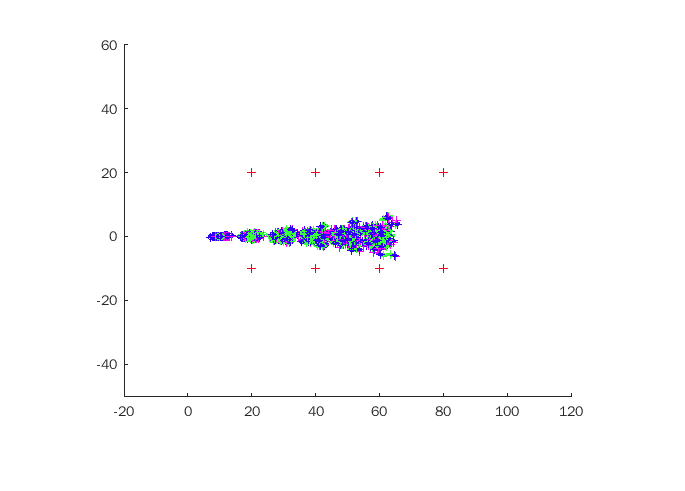
\includegraphics[width=\maxwidth{68.74059207225288em}]{figure_0.png}
\end{center}


\begin{matlabcode}
clc; clear;

load("end_pos_100_runs.mat")
sigma_x = var(end_pos(:,1));
mean_x = mean(end_pos(:,1));

sigma_y = var(end_pos(:,2));
mean_y = mean(end_pos(:,2));

sigma_bearing = var(end_pos(:,3));
mean_bearing = mean(end_pos(:,3));

table(mean_x, sigma_x)
\end{matlabcode}
\begin{matlabtableoutput}
{
\begin{tabular} {|c|c|c|}\hline
\mlcell{ } & \mlcell{mean\_x} & \mlcell{sigma\_x} \\ \hline
\mlcell{1} & \mlcell{59.8330} & \mlcell{5.7994} \\ 
\hline
\end{tabular}
}
\end{matlabtableoutput}
\begin{matlabcode}
table(mean_y, sigma_y)
\end{matlabcode}
\begin{matlabtableoutput}
{
\begin{tabular} {|c|c|c|}\hline
\mlcell{ } & \mlcell{mean\_y} & \mlcell{sigma\_y} \\ \hline
\mlcell{1} & \mlcell{-0.1470} & \mlcell{6.4548} \\ 
\hline
\end{tabular}
}
\end{matlabtableoutput}
\begin{matlabcode}
table(mean_bearing, sigma_bearing)
\end{matlabcode}
\begin{matlabtableoutput}
{
\begin{tabular} {|c|c|c|}\hline
\mlcell{ } & \mlcell{mean\_bearing} & \mlcell{sigma\_bearing} \\ \hline
\mlcell{1} & \mlcell{-0.4008} & \mlcell{25.5979} \\ 
\hline
\end{tabular}
}
\end{matlabtableoutput}
\begin{matlabcode}
table(cov(end_pos))
\end{matlabcode}
\begin{matlabtableoutput}
{
\begin{tabular} {|c|c|c|c|}\hline
\mlcell{ } & \multicolumn{3}{|c|}{\mlcell{Var1}} \\ \hline
\mlcell{1} & \mlcell{5.7994} & \mlcell{-0.5565} & \mlcell{-1.3321} \\ \hline
\mlcell{2} & \mlcell{-0.5565} & \mlcell{6.4548} & \mlcell{10.0519} \\ \hline
\mlcell{3} & \mlcell{-1.3321} & \mlcell{10.0519} & \mlcell{25.5979} \\ 
\hline
\end{tabular}
}
\end{matlabtableoutput}

\begin{par}
\begin{flushleft}
\textbf{Answer.}
\end{flushleft}
\end{par}

\begin{par}
\begin{flushleft}
From the figure and tables seen above, it can be seen that 100 iterations of the first 6 steps forward have been plotted. From this the mean and variance for the x and y positions as well as the bearing have been calculated in the tables above. From these tables it can be seen that the means and variances are all close to their expected values. 
\end{flushleft}
\end{par}

\vspace{10pt}
\hrule
\vspace{10pt}

\matlabheadingtwo{\textbf{3. [5 marks] Reduce the system to use only two (or even one) beacon for simplicity. Configure the code for localisation (so the }$P$\textbf{ matrix for the sensor locations should be set to a small values to indicate that we are very confident about the beacon/landmark locations). Describe qualitatively how the range and heading measurements help constrain the estimate of the robot’s location.}}

\begin{matlabcode}
clc; clear; clf;
for meas_interval = [1 2 6]
    figure
    end_t = 30;
    run("SLAM_2_beacons.m")
    title(['Measurement interval of ', num2str(meas_interval)])
end
\end{matlabcode}
\begin{center}
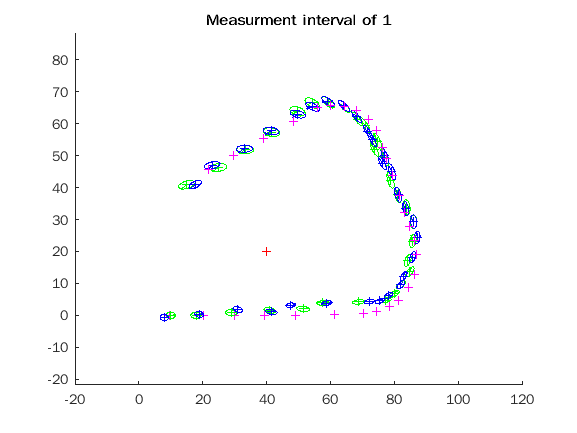
\includegraphics[width=\maxwidth{57.90265930757652em}]{figure_1.png}
\end{center}
\begin{center}
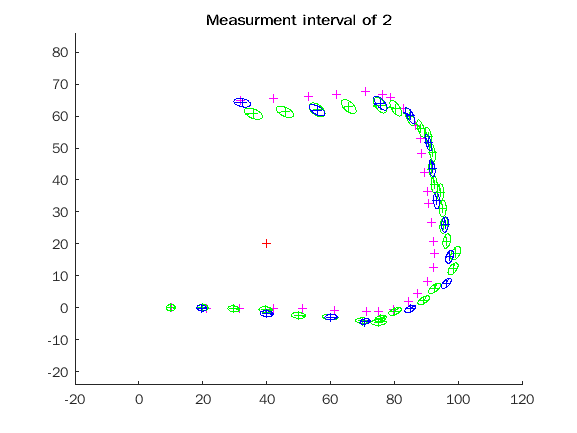
\includegraphics[width=\maxwidth{57.90265930757652em}]{figure_2.png}
\end{center}
\begin{center}
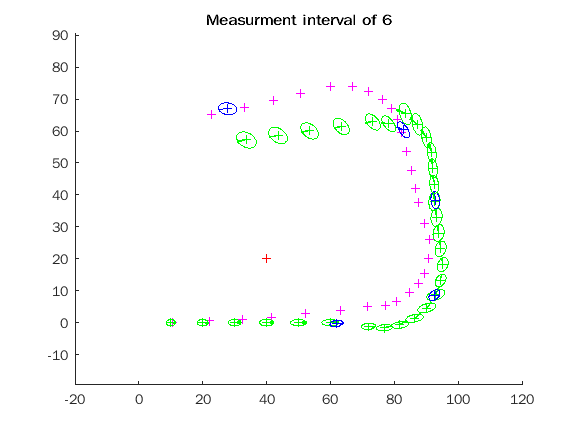
\includegraphics[width=\maxwidth{57.90265930757652em}]{figure_3.png}
\end{center}

\begin{par}
\begin{flushleft}
\textbf{Answer.}
\end{flushleft}
\end{par}

\begin{par}
\begin{flushleft}
From the figures above it can clearly be seen that the measurements of range and heading act to increase the precision and accuracy of the robots estimations of its position, constraining the variance of these estimations. 
\end{flushleft}
\end{par}

\begin{par}
\begin{flushleft}
The is due to the compounding of errors within the estimation when no new measurement are taken to correct them, with larger measurement intervals leading to larger compounded errors and position estimation variances. 
\end{flushleft}
\end{par}

\vspace{10pt}
\hrule
\vspace{10pt}

\matlabheadingtwo{4. [10 marks] As a result of your argument in the previous question, and otherwise, describe how beacons and landmarks should best be spread through an environment. Your discussion should consider the following points.}

\begin{itemize}
\setlength{\itemsep}{-1ex}
   \item{\begin{flushleft} \textit{\textbf{What would be the minimum number of beacons or landmarks that you think would produce adequate performance? How would they be arranged in a space?}} \end{flushleft}}
   \item{\begin{flushleft} \textit{\textbf{Does the number of landmarks / beacons matter? If so discuss any trade-offs in the number of landmarks and the performance of the localisation. }} \end{flushleft}}
   \item{\begin{flushleft} \textit{\textbf{As written the code uses sensor noise that is independent of range. However, in practice we often find that the noise in range measurements increases as the range increases. How would this affect your preferred arrangement of landmarks?}} \end{flushleft}}
   \item{\begin{flushleft} \textit{\textbf{Would your answer change if you could use only range measurements, or only heading measurements?}} \end{flushleft}}
\end{itemize}

\begin{par}
\begin{flushleft}
\textit{\textbf{Answer.}}
\end{flushleft}
\end{par}

\begin{itemize}
    \setlength{\itemsep}{-1ex}
       \item{\begin{flushleft} Technically, the minimum number of beacons required for the SLAM algorithm to work is one, however this will greatly limit the performance. To produce adequate performance from this algorithm I would suggest that at least 3 beacons are located around the robot, ideally spaced equidistant from each other and the robot to allow it to get measurements from different angles. There should also be landmarks distributed throughout the area of the robots intended path to allow for continually reliable speed estimations, as well as allowing the the robot to maintain a minimum distance between itself and the landmarks. \end{flushleft}}
    \end{itemize}
    
    \begin{itemize}
    \setlength{\itemsep}{-1ex}
       \item{\begin{flushleft} By increasing the number of landmarks visible to the robot at any give time, we improve the robustness of the SLAM algorithm, providing more consistent performance across a wide variety of paths and terrains, and allowing for compensation of last landmarks due to obstructions. However the addition of more beacons has diminishing returns after a given point, and serves only to increase the computational complexity and cost of the SLAM algorithm. A possible solution for the added computational cost of adding more beacons would be to select a subset of the currently visible beacons (based on lowest variance from sensor specifications), and only use those for the computation.  \end{flushleft}}
    \end{itemize}
    
    \begin{itemize}
    \setlength{\itemsep}{-1ex}
       \item{\begin{flushleft} If there is range dependant noise in the measurements of distance, it becomes important to ensure that the landmarks are placed within a maximum distance of robot (defined by the acceptable noise level). It may also be recommended that greater confidence is placed in the measurements of beacons that are closer to the robot.  \end{flushleft}}
    \end{itemize}
    
    \begin{itemize}
    \setlength{\itemsep}{-1ex}
       \item{\begin{flushleft} When using only the range measurements for the computation of the slam algorithm, all of the previously discussed answers hold true. It should also be possible to estimate changes in bearing using at least 3 landmarks to look at the direction of movement from the previous to current measurements. On the other hand if heading only measurements are used for the SLAM algorithm, it will be equivalent to removing all beacons as there will be no way to measure their locations. This results in the robot being unable to measure the ground truth of its position and speed, requiring them to be inferred from an internal model of the robot, and measurements such as motor speed and current draw. \end{flushleft}}
    \end{itemize}

\vspace{10pt}
\hrule
\vspace{10pt}

\matlabheadingtwo{\textbf{5. Consider now the full SLAM problem by setting the initial standard deviation of the landmark positions to 10 m. This indicates that the robot has very littel initial confidence in the landmark locations, but is small enough to avoid any issues with data association.}}

\matlabheadingthree{a) [5 marks] Explain how the confidence in the landmark position evolves as a function of time. You should explain qualitatively, but also show representative graphs showing the evolution of the positional certainty. What are the limiting factors in the accuracy with which you can estimate the landmark’s position?}

\begin{par}
\hfill \break
\end{par}

\begin{matlabcode}
clc;clear;clf;

end_t = 30;
run("SLAM_P.m")
\end{matlabcode}
\begin{center}
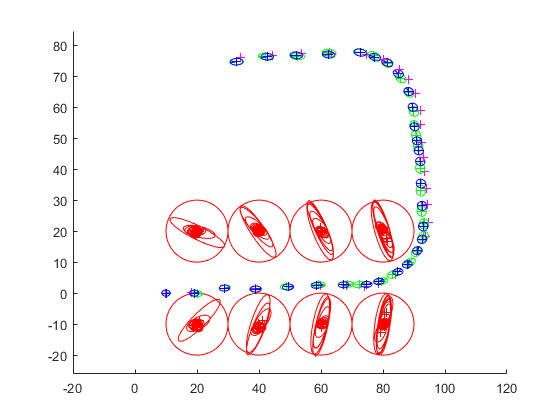
\includegraphics[width=\maxwidth{56.196688409433015em}]{figure_4.png}
\end{center}
\begin{matlabcode}
imshow("static_robot.png")
\end{matlabcode}
\begin{center}
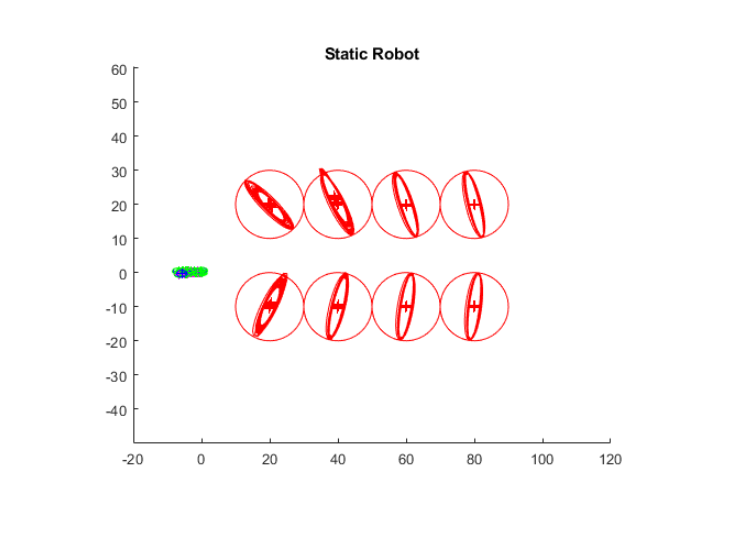
\includegraphics[width=\maxwidth{73.45709984947315em}]{figure_5.png}
\end{center}
\begin{matlabcode}
subplot(121)
plot(P_acc(:, 4:end))
title("Landmark Location Estimate Variance")
subplot(122)
plot(P_acc(:, 1:3))
title("Rover Location Estimate Variance")
\end{matlabcode}
\begin{center}
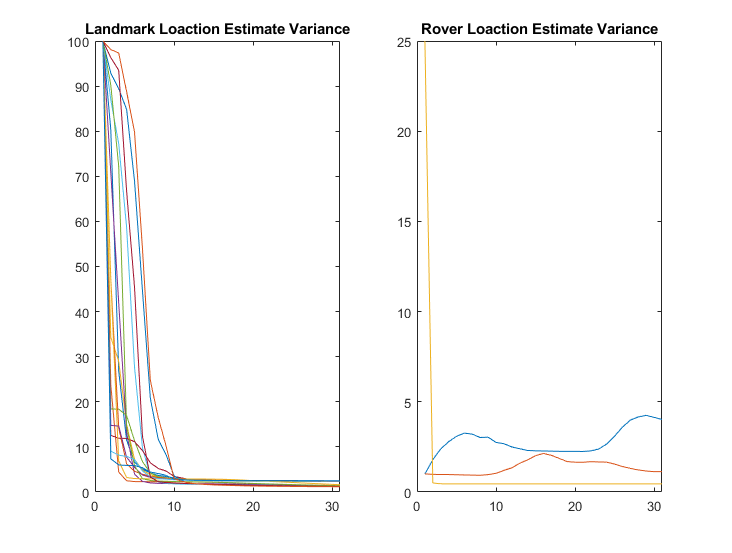
\includegraphics[width=\maxwidth{73.45709984947315em}]{figure_6.png}
\end{center}

\begin{par}
\begin{flushleft}
\textbf{Answer.}
\end{flushleft}
\end{par}

\begin{par}
\begin{flushleft}
It can be seen from both the variance plots above, and the plots of the SLAM simulation that the confidence in the landmark locations increases rapidly to a steady state value. 
\end{flushleft}
\end{par}

\begin{par}
\begin{flushleft}
One of the limiting factors for the estimation of the land mark positions would be both the precision and accuracy of the sensors used in this estimation. 
\end{flushleft}
\end{par}

\begin{par}
\begin{flushleft}
Another limiting factor for this estimation is the robots movement around the marker locations. It can be seen from 'static robot' plot above that if the robot is to remain stationary, then the variance in the estimated beacon locations will remain elliptical perpendicular to the location of the robot. As the robot is to travel around the location of the landmark, this elliptical variance will remain perpendicular to the robot, and as such will decrease.
\end{flushleft}
\end{par}


\matlabheadingthree{b) [5 marks] Imagine that you were given a robot mission that was to perform just mapping. That is, you know perfectly where the robot is at all times (using GPS or similar) and your task is to determine the location of a set of landmarks as quickly as possible. Describe qualitatively the path that you would program the robot to take. Start your description with the case of a single landmark, and then generalise your argument to the case of an arbitrary number of landmarks.}

\begin{par}
\begin{flushleft}
\textbf{Answer.}
\end{flushleft}
\end{par}

\begin{par}
\begin{flushleft}
As discussed in the question above, the major limiting factors for the estimation of landmark locations are the accuracy and precision of the sensors, and the movement of the robot relative to the landmarks. 
\end{flushleft}
\end{par}

\begin{par}
\begin{flushleft}
Due to the elliptical shape of the landmark estimation variance after a measurement has been taken, we can deduced that a path that will take the robot at least ${90}^{\circ }$ around a given landmark (perpendicular to its initial position with relation to the landmark) will provide the lowest variance. 
\end{flushleft}
\end{par}

\begin{par}
\begin{flushleft}
It can also be noted that the precision and accuracy of sensors are often related to the distance of the sensor to the measurement location. Because of this, the path of the robot should preform the ${90}^{\circ }$ encirclement discussed previously, at a distance capable of providing the target measurement variance of the landmark. 
\end{flushleft}
\end{par}

\begin{par}
\begin{flushleft}
These requirements for the robot path can easily be extrapolated to multiple land marks. 
\end{flushleft}
\end{par}


\end{preview}
\end{document}
